% Exemplo: diagrama desenhado no próprio LaTeX com TikZ (fluxo de etapas)
% Compilar: latexmk -pdf figura-tikz.tex          Testado com: abntex2, TikZ, TeX Live 2024 ou mais recente
\documentclass[12pt, a4paper, brazilian]{abntex2}
\usepackage[T1]{fontenc}
\usepackage{tikz}
\usetikzlibrary{arrows.meta, positioning}

\begin{document}

A \autoref{fig:etapas} resume as etapas da pesquisa.

%%BEGIN:figuratikz
\begin{figure}[htbp]
  \caption{Etapas da metodologia}\label{fig:etapas}
  \centering
  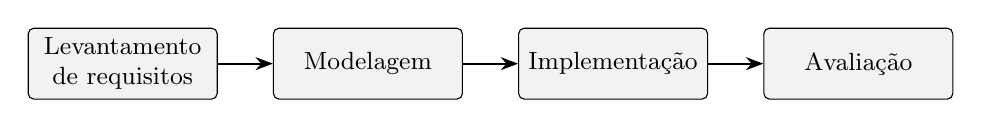
\begin{tikzpicture}[node distance=7mm, font=\small,
      etapa/.style={draw, rounded corners=2pt, minimum height=9mm, minimum width=24mm,
                    align=center, fill=black!5},
      seta/.style={-{Stealth[length=2.2mm]}, thick}]
    \node[etapa] (a) {Levantamento\\de requisitos};
    \node[etapa, right=of a] (b) {Modelagem};
    \node[etapa, right=of b] (c) {Implementação};
    \node[etapa, right=of c] (d) {Avaliação};
    \draw[seta] (a) -- (b);
    \draw[seta] (b) -- (c);
    \draw[seta] (c) -- (d);
  \end{tikzpicture}
  \fonte{Elaborado pelo próprio autor.}
\end{figure}
%%END:figuratikz

\end{document}
